\section{Notion de charge électrique}

La charge est une grandeur extensive. Au niveau microscopique, la charge est portée par des porteurs de charge. Un porteur de charge a une charge quantifiée : $q=ke$ avec $k\in\mathbb{Z}$ et $e=\SI{1.6e-19}{C}$. $e$ s'appelle la charge élémentaire. Un électron porte une charge $q_{e^-}=-e$.

\subsection{Description de la charge}

La répartition des charges peut être modélisée de plusieurs manières.

\subsubsection{Distribution volumique}

$\rho(M,t)$ désigne la densité volumique de charge au point $M$ et à l'instant $t$.

\formule{Charge d'un système en description volumque}
[]
{$$Q=\iiint\rho dV$$}
[
    \begin{itemize}
        \item $Q$ la charge (en \unit{C})
        \item $\rho$ la densité volumique de charge (en \unit{C.m^{-3}})
    \end{itemize}
][o]

\subsubsection{Distribution surfacique}

$\sigma(M,t)$ désigne la densité surfacique de charge au point $M$ et à l'instant $t$.

\formule{Charge d'un système en description surfacique}
[]
{$$Q=\iint\sigma dS$$}
[
    \begin{itemize}
        \item $Q$ la charge (en \unit{C})
        \item $\sigma$ la densité surfacique de charge (en \unit{C.m^{-2}})
    \end{itemize}
][o]

\subsubsection{Distribution linéique}

$\lambda(M,t)$ désigne la densité linéique de charge au point $M$ et à l'instant $t$.

\formule{Charge d'un système en description linéique}
[]
{$$Q=\int\lambda dl$$}
[
    \begin{itemize}
        \item $Q$ la charge (en \unit{C})
        \item $\lambda$ la densité linéique de charge (en \unit{C.m^{-1}})
    \end{itemize}
][o]

\subsubsection{Distribution ponctuelle}

$Q$ désigne la charge d'un objet ponctuel.

\subsection{Charge électrique et force}

\formule{Force d'interaction électrostatique}
[
    Les deux particules sont ponctuelles.
]
{$$\vv{F}_{1/2} = \frac{q_1q_2}{4\pi\epsilon_0}\frac{1}{(M_1M_2)^2}\vv{e}$$
\schema{}{3cm}}
[
    \begin{itemize}
        \item $\vv{F}_{1/2}$ la force exercée par la particule 1 sur la particule 2 (en \unit{N})
        \item $q_1$ la charge de la particule 1 (en \unit{C})
        \item $q_2$ la charge de la particule 2 (en \unit{C})
        \item $\epsilon_0=\SI{8.85e-12}{F.m^{-1}}$ la permittivité diélectrique du vide
        \item $M_1$ le point où se trouve la particule 1
        \item $M_2$ le point où se trouve la particule 2
        \item $\vv{e}=\frac{\vec{M_1M_2}}{\|M_1M_2\|}$ le vecteur unitaire de 1 vers 2
    \end{itemize}
][o]

\flashcard{Force subie par une particule chargée 2 de la part d'une particule chargée 1.}{$$\vv{F}_{1/2} = \frac{q_1q_2}{4\pi\epsilon_0}\frac{1}{(M_1M_2)^2}\vv{e}$$}

La force d'interaction électrostatique est répulsive si les charges sont de même signe.
La force d'interaction électrostatique est attractive si les charges sont de signes différents.

\formule{Champ électrique créé par une particule ponctuelle}
[
    La particule est à l'origine du repère.
]
{$$\vv{E}=\frac{q}{4\pi\epsilon_0}\frac{1}{r^2}\vv{e_r}$$}
[
    \begin{itemize}
        \item $\vv{E}$ le champ électrique (en \unit{V.m^{-1}})
        \item $q$ la charge (en \unit{C})
        \item $\epsilon_0=\SI{8.85e-12}{F.m^{-1}}$ la permittivité diélectrique du vide
        \item $r$ la première coordonnée sphérique (en \unit{m})
    \end{itemize}
][o][o]

\flashcard{Champ électrique créé par une particule ponctuelle.}{$$\vv{E}=\frac{q}{4\pi\epsilon_0}\frac{1}{r^2}\vv{e_r}$$}

\section{Champ et potentiel électriques}

\subsection{Équations de Maxwell}

Le champ électrique obéit aux équations de Maxwell.

\formule{Équation de Maxwell-Gauss}
[]
{$$\divv \vv{E}=\frac{\rho}{\epsilon_0}$$}
[
    \begin{itemize}
        \item $\vv{E}$ le champ électrique (en \unit{V.m^{-1}})
        \item $\rho$ la densité volumique de charge (en \unit{C.m^{-3}})
        \item $\epsilon_0=\SI{8.85e-12}{F.m^{-1}}$ la permittivité diélectrique du vide
    \end{itemize}
][o]

\flashcard{Équation de Maxwell-Gauss}{$$\divv \vv{E}=\frac{\rho}{\epsilon_0}$$}

\formule{Équation de Maxwell-Faraday}
[]
{$$\rot\vv{E}=-\frac{\partial\vv{B}}{\partial t}$$}
[
    \begin{itemize}
        \item $\vv{E}$ le champ électrique (en \unit{V.m^{-1}})
        \item $\vv{B}$ le champ magnétique (en \unit{T})
    \end{itemize}
][o]

\flashcard{Équation de Maxwell-Faraday}{$$\rot\vv{E}=-\frac{\partial\vv{B}}{\partial t}$$}

\subsection{Potentiel électrique}

En régime stationnaire, le potentiel électrique peut s'écrire comme un gradient.

\formule{Potentiel électrique}
[En régime stationnaire]
{$$\vv{E}=-\grad V$$}
[
    \begin{itemize}
        \item $\vv{E}$ le champ électrique (en \unit{V.m^{-1}})
        \item $V$ le potentiel électrique (en \unit{V})
    \end{itemize}
][o][o]

\flashcard{Lien entre potentiel électrique et champ électrique.}{$$\vv{E}=-\grad v$$}

Cette équation définit le potentiel électrique.

Comme $\grad K=\vv{0}$, le potentiel électrique est défini à une constante près. On choisit arbitrairement la valeur du potentiel électrique en un point.

\formule{Circulation de $\vv{E}$}
[En régime stationnaire]
{$$\int_A^B\vv{E}.\vv{dl}=V_A-V_B$$}
[
    \begin{itemize}
        \item $A$ et $B$ deux points de l'espace
        \item $\vv{E}$ le champ électrique (en \unit{V.m^{-1}})
        \item $V_A$ le potentiel électrique au point $A$ (en \unit{V})
        \item $V_B$ le potentiel électrique au point $B$ (en \unit{V})
    \end{itemize}
][o][o]

\flashcard{Circulation du champ électrique}{$$\int_A^B\vv{E}.\vv{dl}=V_A-V_B$$}

\colle{Énoncer l'équation de Maxwell-Faraday, en déduire qu'en régime stationnaire, $\vv{E}=-\vv{\text{grad}}V$ puis exprimer la circulation du champ électrique.}

\subsection{Équation de Poisson}

\formule{Équation de Poisson}
[En régime stationnaire]
{$$\Delta V=-\frac{\rho}{\epsilon_0}$$}
[
    \begin{itemize}
        \item $\Delta$ le laplacien scalaire
        \item $V$ le potentiel électrique (en \unit{V})
        \item $\rho$ la densité volumique de charge (en \unit{C.m^{-3}})
        \item $\epsilon_0=\SI{8.85e-12}{F.m^{-1}}$ la permittivité diélectrique du vide
    \end{itemize}
][o][o]

\flashcard{Équation de Poisson vérifiée par le potentiel électrique}{$$\Delta V=-\frac{\rho}{\epsilon_0}$$}

\formule{Équation de Laplace}
[\begin{itemize}
    \item en régime stationnaire
    \item dans les zones vides de charges
\end{itemize}]
{$$\Delta V=0$$}
[
    \begin{itemize}
        \item $\Delta$ le laplacien scalaire
        \item $V$ le potentiel électrique (en \unit{V})
    \end{itemize}
][o][o]

\flashcard{Équation de Laplace vérifiée par le potentiel électrique dans le vide}{$$\Delta V=0$$}

\colle{Énoncer les équations de Maxwell-Gauss et Maxwell-Faraday puis établir les équations de Poisson et de Laplace vérifiées par le potentiel électrique.}

\subsection{Topographie des cartes de champ}

\subsubsection{Tubes de champ en absence de sources}

Une ligne de champ est une courbe qui est en tout point à un champ vectoriel.
\schema{Ligne de champ}{4cm}

Un tube de champ est un ensemble de lignes de champ s'appuyant sur une courbe fermée.
\schema{Tube de champ}{4cm}

\formule{Conservativité du flux de $\vv{E}$}
[
    \begin{itemize}
        \item en régime stationnaire
        \item dans les zones vides de charges
    \end{itemize}
]
{Le flux de $\vv{E}$ est le même sur chaque section d'un tube de champ.}
[$\vv{E}$ le champ électrique (en \unit{V.m^{-1}})\schema{}{3cm}][o][o]

\flashcard{Conditions pour que $\vv{E}$ soit à flux conservatif}{en régime stationnaire, dans les zones vides de charges}

Un rétrécissement d'un tube de champ s'accompagne donc d'une augmentation de la norme du champ électrique.

\subsubsection{De l'un à l'autre}

\formule{Lien entre cartes de champ électrique et de potentiel électrique}
[En régime stationnaire]
{
    \begin{itemize}
        \item Les lignes de champ sont orthogonales aux équipotentielles
        \item $\vv{E}$ pointe dans le sens où $V$ diminue le plus vite
        \item plus $\|\vv{E}\|$ est grand, plus les équipotentielles sont resserrées
    \end{itemize}
}[][o]

\flashcard{Lien entre cartes de champ électrique et de potentiel électrique}{Les lignes de champ sont orthogonales aux équipotentielles ; $\vv{E}$ pointe dans le sens où $V$ diminue le plus vite ; plus $\vv{E}$ est grand, plus les équipotentielles sont resserrées}

\application{Tracer des lignes de champ électrique sur les cartes représentant des équipententielles.
\\\begin{tikzpicture}[scale=0.7]
    \draw (0,0) circle (0.5) (0,0.5) node[above] {\SI{0}{V}};
    \draw (0,0) circle (1) (0,1) node[above] {\SI{5}{V}};
    \draw (0,0) circle (2) (0,2) node[above] {\SI{10}{V}};
    \draw (0,0) circle (4) (0,4) node[above] {\SI{15}{V}};

    \begin{scope}[xshift=10cm]
        \draw (0.5,-3) -- (0.5,3) node[above] {\SI{30}{V}};
        \draw (1,-3) node[below] {\SI{20}{V}} -- (1,3);
        \draw (2,-3) -- (2,3) node[above] {\SI{10}{V}};
        \draw (4,-3) node[below] {\SI{0}{V}} -- (4,3);
    \end{scope}
\end{tikzpicture}}

\application{Tracer des équipotentielles sur la carte représentant des lignes de champ.
\\\tikzset{
  on each segment/.style={
    decorate,
    decoration={
      show path construction,
      moveto code={},
      lineto code={
        \path [#1]
        (\tikzinputsegmentfirst) -- (\tikzinputsegmentlast);
      },
      curveto code={
        \path [#1] (\tikzinputsegmentfirst)
        .. controls
        (\tikzinputsegmentsupporta) and (\tikzinputsegmentsupportb)
        ..
        (\tikzinputsegmentlast);
      },
      closepath code={
        \path [#1]
        (\tikzinputsegmentfirst) -- (\tikzinputsegmentlast);
      },
    },
  },
  % style to add an arrow in the middle of a path
  mid arrow/.style={postaction={decorate,decoration={
        markings,
        mark=at position .5 with {\arrow[#1]{stealth}}
      }}},
}
\begin{tikzpicture}[scale=0.7]
    \draw[postaction={on each segment={mid arrow=black}}] (0,1) ..controls (4,1) and (6,1).. (10,4)
        (0,0.5) ..controls (4,0.5) and (6,0.5).. (10,2)
        (0,0) -- (10,0)
        (0,-0.5) ..controls (4,-0.5) and (6,-0.5).. (10,-2)
        (0,-1) ..controls (4,-1) and (6,-1).. (10,-4)
    ;
\end{tikzpicture}}

\application{Déterminer la valeur, la direction et le sens du champ électrique aux points $M_1$ et $M_2$ en utilisant la carte des équipotentielles.\\\begin{tikzpicture}
    \draw (0,-2) --++ (0,4) node[above] {\SI{0}{V}}
        (0.2,-2) --++ (0,4)
        (0.4,-2) --++ (0,4)
        (0.6,-2) --++ (0,4)
        (1,-2) --++ (0,4)
        (1.3,-2) --++ (0,4) node[above] {\SI{5}{V}}
        (1.7,-2) --++ (0,4)
        (2.2,-2) --++ (0,4)
        (2.8,-2) --++ (0,4)
        (3.5,-2) --++ (0,4)
        (4.4,-2) --++ (0,4) node[above] {\SI{10}{V}}
        (5.4,-2) --++ (0,4)
        (6.4,-2) --++ (0,4)
        (7.4,-2) --++ (0,4)
        (8.4,-2) --++ (0,4)
        (9.4,-2) --++ (0,4) node[above] {\SI{15}{V}};
    \fill (0.2,0) circle (0.05) node[above] {$M_1$};
    \fill (8.4,0) circle (0.05) node[above] {$M_2$};
\end{tikzpicture}}

\subsection{Linéarité}

Les équations de Maxwell sont linéaires, il est donc possible d'utiliser le théorème de superposition.

\formule{Théorème de superposition}
[]
{Si les distributions de charge $\rho_1$ et $\rho_2$ créent respectivement les champ électrique $\vv{E_1}$ et $\vv{E_2}$, alors la distribution $\rho_1+\rho_2$ crée le champ $\vv{E_1}+\vv{E_2}$.}[][o]

\section{Théorème de Gauss}

\subsection{Symétries du champ électrique}

L'existence de symétries dans la distribution de charge contraint le champ électrique associé.

\formule{Principe de Curie}
[]
{Lorsque des causes produisent des effets, les symétries de causes doivent se retrouver dans leurs effets.}[][o]

\formule{Plans de symétries et champ électrique}
[]
{Le champ électrique est inclus dans les plans de symétrie de la distribution de charge.}
[][o][o]

\flashcard{Rapport du champ électrique aux plans de symétrie}{Le champ électrique est inclus dans les plans de symétrie de la distribution de charge}

\application{On considère une boule uniformément chargée. Déterminer la direction du champ électrique en tout point de l'espace.}

Si, pour chaque couple de points symétriques l'un de l'autre par un plan, la distribution de charge est opposée en ces points, le plan est appelé plan d'antisymétrie.

\formule{Plans d'antisymétries et champ électrique}
[]
{Le champ électrique est orthogonal aux plans d'antisymétrie de la distribution de charge.}
[][o][o]

\flashcard{Rapport du champ électrique aux plans d'antisymétrie}{Le champ électrique est orthogonal aux plans d'antisymétrie de la distribution de charge.}

\application{On considère deux armatures planes se faisant face, de charges opposées. Déterminer la direction du champ électrique dans le plan médiateur des armatures.\schema{}{3cm}}

\subsection{Invariances du champ électrique}

Un champ est invariant par une transformation si cette transformation laisse ce champ inchangé.

L'existence d'invariances dans la distribution de charge contraint le champ électrique associé.

\formule{Principe de Curie}
[]
{Lorsque des causes produisent des effets, les invariances de causes doivent se retrouver dans leurs effets.}[][o]

\flashcard{Lien entre les invariances de $\vv{E}$ et de la distribution de charge}{$\vv{E}$ a les mêmes invariances que la distribution de charge.}

\application{De quelles variables d'espace dépend le champ électrique dans les situations suivantes.
\begin{enumerate}
    \item boule uniformément chargée de densité volumique de charge $\rho$
    \item plan infini uniformément charge de densité surfacique de charge $\sigma$
    \item fil infini infiniment fin uniformément chargé de densité linéique de charge $\lambda$
\end{enumerate}
}

\subsection{Théorème de Gauss}

\formule{Théorème de Gauss}
[En régime stationnaire]
{$$\oiint_S \vv{E}.\vv{dS}=\frac{Q_\text{int}}{\epsilon_0}$$}
[
    \begin{itemize}
        \item $S$ une surface fermée orientée vers l'extérieur
        \item $\vv{E}$ le champ électrique (en \unit{V.m^{-1}})
        \item $Q_\text{int}$ la charge électrique contenue à l'intérieure de $S$ (en \unit{C})
        \item $\epsilon_0$ la permittivité diélectrique du vide (en \unit{F.m^{-1}})
    \end{itemize}
][o][o]

\flashcard{Théorème de Gauss}{$$\oiint_S \vv{E}.\vv{dS}=\frac{Q_\text{int}}{\epsilon_0}$$}

\colle{Énoncer l'équation de Maxwell-Gauss et démontrer le théorème de Gauss.}

\application{Déterminer le champ électrique créé par une particule ponctuelle de charg $q$.}
\colle{Déterminer le champ électrique créé par une particule ponctuelle de charg $q$.}

\application{Déterminer le champ électrique créé par une boule de rayon $R$ uniformément chargée de densité volumique de charge $\rho$.}
\colle{Déterminer le champ électrique créé par une boule uniformément chargée de densité volumique de charge $\rho$.}

\application{Déterminer le champ électrique créé par un cylindre (plein) de rayon $R$, infiniment haut, uniformément chargé de densité volumique de charge $\rho$.}
\colle{Déterminer le champ électrique créé par un cylindre (plein) uniformément chargé de densité volumique de charge $\rho$.}

\application{Déterminer le champ électrique créé par un plan infini uniformément chargé de densité surfacique de charge $\sigma$.}
\colle{Déterminer le champ électrique créé par un plan infini uniformément chargé de densité surfacique de charge $\sigma$.}

\subsection{Analogie avec le champ de gravité}

Champ électrique et champ gravitationnel sont analogues.

\begin{center}
    \begin{tabular}{c|c|c}
        & électrostatique & gravitation\\
        \hline
        Grandeur portée par une particule & charge $q$ (en \unit{C}) & masse $m$ (en \unit{kg})\\[.5cm]
        Force & $\vv{F}_{1/2}=\dfrac{q_1q_2}{4\pi\epsilon_0}\dfrac{1}{(M_1M_2)^2}\vv{e}$ & $\vv{F}_{1/2}=-\mathcal{G}m_1m_2\dfrac{1}{(M_1M_2)^2}\vv{e}$\\[.5cm]
        & $=q_2\vv{E}(M_2)$ & $=m_2\vv{g}(M_2)$\\[.5cm]
        Champ & $\vv{E}$ (\unit{V.m^{-1}}) & $\vv{g}$ (\unit{m.s^{-2}})\\[.2cm]
        & $\dfrac{1}{4\pi\epsilon_0}$ & $-\mathcal{G}$
    \end{tabular}
\end{center}

\formule{Théorème de Gauss gravitationnel}
[]
{$$\oiint\vv{g}.\vv{dS}=-4\pi\mathcal{G}M_\text{int}$$}
[
    \begin{itemize}
        \item $S$ une surface fermée orientée vers l'extérieur
        \item $\vv{g}$ le champ gravitationnel (en \unit{m.s^{-2}})
        \item $M_\text{int}$ la masse contenue à l'intérieure de $S$ (en \unit{kg})
        \item $\mathcal{G}=\SI{6.6e-11}{m^3.kg^{-1}.s^{-2}}$ la constante gravitationnelle\footnote{aussi appelée constante universelle de gravitation} (en \unit{m^3.kg^{-1}.s^{-2}})
    \end{itemize}
][o][o]

\flashcard{Théorème de Gauss gravitationnel}{$$\oiint\vv{g}.\vv{dS}=-4\pi\mathcal{G}M_\text{int}$$}
\colle{Dresser les analogies entre les champs électrique et gravitationnel. Énoncer le théorème de Gauss gravitationnel.}

\application{La Terre a une masse $m_T=\SI{6.0e24}{kg}$ et un rayon de $R=\SI{6.3e3}{km}$. Déterminer le champ gravitationnel créé par la Terre dans tout l'espace en supposant sa masse volumique uniforme.}
\colle{Déterminer le champ gravitationnel créé par une boule de masse volumique uniforme $\mu$.}

\section{Condensateur plan}

\subsection{Champ électrique}

\formule{Champ électrique dans un condensateur}
[
    \begin{itemize}
        \item en régime stationnaire
        \item les effets de bord sont négligés
        \item le condensateur est constitué du deux armatures planes en regard
        \item les armatures sont séparées de vide
        \item les armatures ont des charges opposées
        \item les armatures sont uniformément chargées
    \end{itemize}
]
{$$\vv{E}=\left\lbrace
    \begin{aligned}
        \frac{Q}{\epsilon_0S}\vv{n} &\text{ entre les armatures}\\
        \vv{0} &\text{ ailleurs}
    \end{aligned}\right.$$}
[
    \schema{}{3cm}
    \begin{itemize}
        \item $\vv{E}$ le champ électrique (en \unit{V.m^{-1}})
        \item $Q$ la charge d'une armature (en \unit{C})
        \item $\epsilon_0$ la permittivité diélectrique du vide (en \unit{F.m^{-1}})
        \item $\vv{n}$ un vecteur unitaire allant de l'armature chargée positivement vers celle chargée négativement
        \item $S$ la surface de chacune des armatures (en \unit{m^2})
    \end{itemize}
][][o]

\subsection{Capacité}

\formule{Capacité d'un condensateur plan}
[
    \begin{itemize}
        \item en régime stationnaire
        \item les effets de bord sont négligés
        \item le condensateur est constitué du deux armatures planes identiques en regard
        \item les armatures sont séparées de vide
        \item les armatures ont des charges opposées
    \end{itemize}
]
{$$C=\frac{\epsilon_0S}{e}$$}
[
    \begin{itemize}
        \item $C$ la capacité du condensateur (en \unit{F})
        \item $S$ la surface de chacune des armatures (en \unit{m^2})
        \item $\epsilon_0$ la permittivité diélectrique du vide (en \unit{F.m^{-1}})
        \item $e$ la distance entre les armatures (en \unit{m})
    \end{itemize}
][o][o]

\subsection{Influence de la permittivité}

Lorsque l'espace entre les armatures n'est pas vide mais occupé par un isolant, il faut prendre en compte sa permittivité.

\formule{Capacité d'un condensateur plan}
[
    \begin{itemize}
        \item en régime stationnaire
        \item les effets de bord sont négligés
        \item le condensateur est constitué du deux armatures planes identiques en regard
        \item les armatures ont des charges opposées
    \end{itemize}
    \schema{}{3cm}
]
{$$C=\frac{\epsilon S}{e}$$}
[
    \begin{itemize}
        \item $C$ la capacité du condensateur (en \unit{F})
        \item $S$ la surface de chacune des armatures (en \unit{m^2})
        \item $\epsilon=\epsilon_r\epsilon_0$ la permittivité diélectrique de l'isolant (en \unit{F.m^{-1}})
        \item $\epsilon_r$ la permittivité diélectrique relative de l'isolant (sans unité)
        \item $\epsilon_0$ la permittivité diélectrique du vide (en \unit{F.m^{-1}})
        \item $e$ la distance entre les armatures (en \unit{m})
    \end{itemize}
][][o]

\flashcard{Capacité d'un condensateur}{$$C=\frac{\epsilon S}{e}$$ avec $\epsilon=\epsilon_0\epsilon_r$}
\colle{Établir le champ électrique entre les armatures d'un condensateur plan. En déduire la capacité. Généraliser au cas où l'isolant entre les armatures n'est pas du vide.}

\application{
    \begin{wrapfigure}{r}{1.5cm}
        \centering
        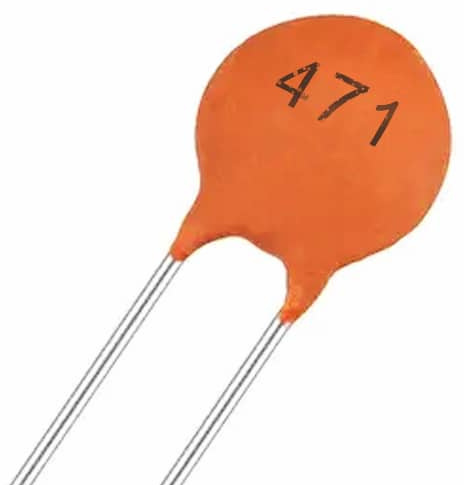
\includegraphics[width=1.5cm]{images/condensateur.jpg}
    \end{wrapfigure}
    Un condensateur céramique de capacité \SI{470}{pF} comporte un matériau diélectrique (une céramique) de permittivité diélectrique relative \SI{20}{} et d'épaisseur \SI{1}{\micro m}. Déterminer le diamètre des armatures.
}

\subsection{Aspect énergétique}

L'énergie stockée dans un condensateur est $\mathcal{E}=\frac{1}{2}CU^2$.

\formule{Densité volumique d'énergie électrostatique}
[Dans le vide]
{$$w=\frac{1}{2}\epsilon_0E^2$$}
[
    \begin{itemize}
        \item $w$ la densité volumique d'énergie électrostatique (en \unit{J.m^{-3}})
        \item $\epsilon_0$ la permittivité diélectrique du vide (en \unit{F.m^{-1}})
        \item $E$ le champ électrique (en \unit{V.m^{-1}})
    \end{itemize}
][o][o]

\flashcard{Densité volumique d'énergie électrostatique}{$$w=\frac{1}{2}\epsilon_0E^2$$}

\application{Déterminer l'énergie électrostatique totale dans tout l'espace pour une boule uniformément chargée de densité volumique de charge $\rho$ et de rayon $R$.}
